\begin{frame}
\end{frame}

\begin{frame}{Deep Learning: Current State of The Art in ML}
\protect\hypertarget{deep-learning-current-state-of-the-art-in-ml}{}
\begin{itemize}
\tightlist
\item
  Breakthroughs in broad range of challenging domain problems

  \begin{itemize}
  \tightlist
  \item
    computer vision, language understanding, complex control, protein
    structure prediction, \ldots{}
  \end{itemize}
\end{itemize}

\center{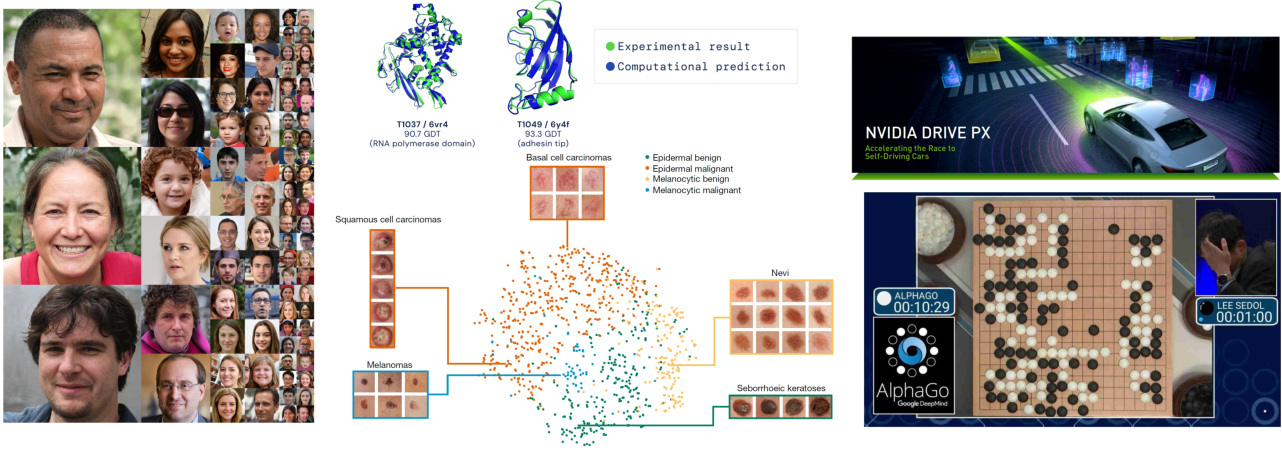
\includegraphics[width=\textwidth]{../images/Overview_Applications.pdf}}

\footnote<.->{\tiny Karras et al., 2019; Esteva et al., 2017; Jumper et
  al., 2020}
\end{frame}

\begin{frame}{Deep Learning: Current State of The Art in ML}
\protect\hypertarget{deep-learning-current-state-of-the-art-in-ml-1}{}
\begin{itemize}
\tightlist
\item
  Consistently outperforming all other ML methods on large dataset
  benchmarks

  \begin{itemize}
  \tightlist
  \item
    ImageNet-1k (1.4 M samples, 224x224, 0.4 TB), FFHQ (70k samples,
    1024x1024, 2.5 TB), \ldots{}
  \item
    Recent development: very large scale multi-modal (language-vision)
    datasets: LAION-400M/5B (400M/5B image-text pairs)
  \end{itemize}
\end{itemize}

\center{\includegraphics[width=0.7\textwidth]{../images/ImageNet_Outperforming.pdf}}
\end{frame}

\begin{frame}{Deep Learning: Current State of The Art in ML}
\protect\hypertarget{deep-learning-current-state-of-the-art-in-ml-2}{}
\begin{itemize}
\tightlist
\item
  Consistently outperforming all other ML methods on large dataset
  benchmarks

  \begin{itemize}
  \tightlist
  \item
    convolutional and transformer networks predominant
  \end{itemize}
\end{itemize}

\center{\includegraphics[width=0.9\textwidth]{../images/ImageNet_Outperforming_2.pdf}}
\end{frame}

\begin{frame}{Deep Learning: Current State of The Art in ML}
\protect\hypertarget{deep-learning-current-state-of-the-art-in-ml-3}{}
\begin{itemize}
\tightlist
\item
  Self-supervised multi-modal (language-vision) learning: no explicit
  labels required

  \begin{itemize}
  \tightlist
  \item
    openAI CLIP: very strong zero- and few-shot transfer across various
    targets
  \item
    requires very large data for pre-training (eg. publicly available
    LAION-400M/5B)
  \item
    self-supervised learning from weakly aligned image-text pairs:
    public Internet as scalable data source
  \end{itemize}
\end{itemize}

\center{\includegraphics[width=\textwidth]{../images/CLIP_Zero_Shot_Few_Shot_Self-Supervised_mod.pdf}}

\footnote<.->{\tiny Radford et al., ICML, 2021}
\end{frame}

\begin{frame}{Deep Learning: Current State of The Art in ML}
\protect\hypertarget{deep-learning-current-state-of-the-art-in-ml-4}{}
\begin{itemize}
\tightlist
\item
  Consistently outperforming all other ML methods

  \begin{itemize}
  \tightlist
  \item
    AlphaFold 2: Transformer networks (predominant in natural language
    processing)
  \item
    Big Fantastic Database (BFD): 2.4B protein sequences, 0.27 TB
  \end{itemize}
\end{itemize}

\center{\includegraphics[width=\textwidth]{../images/CASP_Outperforming.png}}

\footnote<.->{\tiny Jumper et al., Nature, 2021}
\end{frame}

\begin{frame}{Deep Learning is Supercomputing}
\protect\hypertarget{deep-learning-is-supercomputing}{}
\begin{itemize}
\tightlist
\item
  Training of models requires accelerators

  \begin{itemize}
  \tightlist
  \item
    GPUs (currently NVIDIA dominant), TPUs (Google)
  \item
    GPUs: generic deep learning hardware

    \begin{itemize}
    \tightlist
    \item
      parallelizing matrix/tensor operations via vectorization
    \end{itemize}
  \end{itemize}
\end{itemize}

\center{\includegraphics[width=\textwidth]{../images/GPU_TPU.pdf}}
\end{frame}

\begin{frame}{Deep Learning is Supercomputing}
\protect\hypertarget{deep-learning-is-supercomputing-1}{}
\begin{itemize}
\tightlist
\item
  Training of models requires accelerators

  \begin{itemize}
  \tightlist
  \item
    spezialized hardware, eg. in-memory computing chips
  \item
    Graphcore IPU: Colossus MK2
  \item
    Cerebras: Wafer Scale Engine 2 (850k cores!)
  \end{itemize}
\end{itemize}

\center{\includegraphics[width=\textwidth]{../images/Graphcore_Cerebras.pdf}}
\end{frame}

\begin{frame}{Deep Learning is Supercomputing}
\protect\hypertarget{deep-learning-is-supercomputing-2}{}
\begin{itemize}
\tightlist
\item
  Most breakthroughs require heavy compute power, using many
  accelerators simultaneously

  \begin{itemize}
  \tightlist
  \item
    GPT-3: natural language generation, language understanding
  \item
    CLIP, DALL-E 2, Stable Diffusion: image understanding and image
    generation\\
  \item
    AlphaFold 2: protein structure prediction
  \item
    AlphaZero, MuZero: learning control in highly dimensional
    state-action spaces
  \end{itemize}
\end{itemize}

\center{\includegraphics[width=\textwidth]{../images/GPT-3_AlphaFold2_HighRes.png}}
\end{frame}

\begin{frame}{Deep Learning is Supercomputing}
\protect\hypertarget{deep-learning-is-supercomputing-3}{}
\begin{itemize}
\tightlist
\item
  Many recent breakthroughs require heavy compute power, using many
  accelerators simultaneously

  \begin{itemize}
  \tightlist
  \item
    GPT-3: natural language generation, language understanding
  \item
    CLIP, DALL-E: image understanding and image generation\\
  \item
    AlphaFold 2: protein structure prediction
  \item
    AlphaZero, MuZero: learning control in highly dimensional
    state-action spaces
  \end{itemize}
\end{itemize}

\center{\includegraphics[width=0.8\textwidth]{../images/JUWELS_Booster.pdf}}
\end{frame}

\begin{frame}{Deep Learning is Supercomputing}
\protect\hypertarget{deep-learning-is-supercomputing-4}{}
\begin{columns}[T]
\begin{column}{0.4\textwidth}
\begin{itemize}
\tightlist
\item
  GPT-3: natural language generation, language understanding

  \begin{itemize}
  \tightlist
  \item
    1 model: 175 billion weight parameters
  \item
    compare:

    \begin{itemize}
    \tightlist
    \item
      AlexNet, winner ILSRVC 2012 -- 60M
    \item
      ResNet-50, winner ILSRVC 2015 -- 25M
    \item
      CLIP ViT L/14, multi-modal learning, 2021 - 600M
    \end{itemize}
  \end{itemize}
\end{itemize}
\end{column}

\begin{column}{0.6\textwidth}
\vspace*{2cm}
\center{\includegraphics[width=0.9\textwidth]{../images/JUWELS_Booster.pdf}}
\end{column}
\end{columns}
\end{frame}

\begin{frame}{Deep Learning is Supercomputing}
\protect\hypertarget{deep-learning-is-supercomputing-5}{}
\begin{columns}[T]
\begin{column}{0.4\textwidth}
\begin{itemize}
\tightlist
\item
  GPT-3: natural language generation, language understanding

  \begin{itemize}
  \tightlist
  \item
    1 model: \(\approx\) 350 GB memory for training
  \item
    splitting over 22 V100 GPUs required for one model to run
  \end{itemize}
\end{itemize}
\end{column}

\begin{column}{0.6\textwidth}
\vspace*{2cm}
\center{\includegraphics[width=0.9\textwidth]{../images/JUWELS_Booster.pdf}}
\end{column}
\end{columns}
\end{frame}

\begin{frame}{Deep Learning is Supercomputing}
\protect\hypertarget{deep-learning-is-supercomputing-6}{}
\begin{columns}[T]
\begin{column}{0.4\textwidth}
\begin{itemize}
\tightlist
\item
  GPT-3: natural language generation, language understanding

  \begin{itemize}
  \tightlist
  \item
    1 model full training:\\
    \(\approx\) \(3.14\cdot 10^{23}\) FLOPS
  \item
    \(\approx\) 355 years for V100;\\
    \(\approx\) 90 years for A100
  \end{itemize}
\end{itemize}
\end{column}

\begin{column}{0.6\textwidth}
\vspace*{2cm}
\center{\includegraphics[width=0.9\textwidth]{../images/JUWELS_Booster.pdf}}
\end{column}
\end{columns}
\end{frame}

\begin{frame}{Deep Learning is Supercomputing}
\protect\hypertarget{deep-learning-is-supercomputing-7}{}
\begin{columns}[T]
\begin{column}{0.4\textwidth}
\begin{itemize}
\tightlist
\item
  GPT-3: natural language generation, language understanding

  \begin{itemize}
  \tightlist
  \item
    1 model full training:\\
    \(\approx\) \(3.14\cdot 10^{23}\) FLOPS
  \item
    \(\approx\) 16 days if scaled well with \(2\,000\) A100 GPUs on
    JUWELS Booster
  \end{itemize}
\end{itemize}
\end{column}

\begin{column}{0.6\textwidth}
\vspace*{2cm}
\center{\includegraphics[width=0.9\textwidth]{../images/JUWELS_Booster.pdf}}
\end{column}
\end{columns}
\end{frame}

\begin{frame}{Deep Learning is Supercomputing}
\protect\hypertarget{deep-learning-is-supercomputing-8}{}
\begin{columns}[T]
\begin{column}{0.4\textwidth}
\begin{itemize}
\tightlist
\item
  CLIP: self-supervised image-text learning, strong zero-shot transfer

  \begin{itemize}
  \tightlist
  \item
    openCLIP ViT g/14, 1480 A100 GPUs
  \item
    8 days on 34B samples from LAION-2B
  \end{itemize}

  → for training a single language-vision model
\end{itemize}
\end{column}

\begin{column}{0.6\textwidth}
\vspace*{2cm}
\center{\includegraphics[width=0.9\textwidth]{../images/JUWELS_Booster.pdf}}
\end{column}
\end{columns}
\end{frame}

\begin{frame}{Deep Learning is Supercomputing}
\protect\hypertarget{deep-learning-is-supercomputing-9}{}
\begin{columns}[T]
\begin{column}{0.4\textwidth}
\begin{itemize}
\tightlist
\item
  AlphaFold 2: protein structure prediction

  \begin{itemize}
  \tightlist
  \item
    128 TPUs
  \item
    few weeks
  \end{itemize}

  → for training a single model
\end{itemize}
\end{column}

\begin{column}{0.6\textwidth}
\vspace*{2cm}
\center{\includegraphics[width=0.9\textwidth]{../images/JUWELS_Booster.pdf}}
\end{column}
\end{columns}
\end{frame}

\begin{frame}{Deep Learning is Supercomputing}
\protect\hypertarget{deep-learning-is-supercomputing-10}{}
\begin{itemize}
\tightlist
\item
  Foundation models: transferable models pre-trained on large generic
  data

  \begin{itemize}
  \tightlist
  \item
    transfer across domains specific smaller datasets and tasks
  \item
    strong, efficient transfer: requires large pre-trained models
  \end{itemize}
\end{itemize}

\center{\includegraphics[width=0.8\textwidth]{../images/Pretrain_Transfer_Foundation_Model_mod.pdf}}
\end{frame}

\begin{frame}{Deep Learning is Supercomputing}
\protect\hypertarget{deep-learning-is-supercomputing-11}{}
\begin{itemize}
\tightlist
\item
  Investigating strong transferable models: pre-training on a large
  dataset, requires a large machine

  \begin{itemize}
  \tightlist
  \item
    a rather compact ResNet-50 on ImageNet-1k: still
    \textbf{\(\boldsymbol{\approx}\) 20 hours} for full training (single
    V100)
  \item
    can be done in \textbf{a few minutes} if using thousands of GPU
  \item
    High Performance Computing (HPC): many strong compute nodes, fast
    interconnect (InfiniBand)
  \end{itemize}
\end{itemize}

\center{\includegraphics[width=0.8\textwidth]{../images/JUWELS_Booster.pdf}}
\end{frame}

\begin{frame}{Deep Learning: Basics Recap}
\protect\hypertarget{deep-learning-basics-recap}{}
\begin{block}{Machine Learning}
\protect\hypertarget{machine-learning}{}
Optimizing loss (objective) of a (complex) model \(f\) using (a lot of)
data \(\mathcal{D}\)
\end{block}

\begin{itemize}
\tightlist
\item
  a (complex) model: function (or distribution) family
  \(f(X;\boldsymbol{\theta})\) (\(p(X;\boldsymbol{\theta})\))

  \begin{itemize}
  \tightlist
  \item
    parameters \(\boldsymbol{\theta}\) (often \(\mathbf{W}\) is used)
    are to adapt (``fit'') given the data samples
    \(X \in \mathcal{\hat{D}}\)
  \end{itemize}
\item
  optimization:

  \begin{itemize}
  \tightlist
  \item
    defining a loss
    \(\mathcal{L}(f(X;\boldsymbol{\theta}),\mathcal{\hat{D}})\)
  \item
    loss \(\mathcal{L}\): measure of quality (``fit'') of
    \(f(X;\boldsymbol{\theta})\) in terms of a task solution on
    \(\mathcal{\hat{D}}\)
  \item
    seeking to minimize \(\mathcal{L}(f,\mathcal{\hat{D}})\) with
    respect to all possible \(\mathcal{\hat{D}} \sim P(\mathcal{D})\)!
  \end{itemize}
\end{itemize}

\center{\includegraphics[width=\textwidth]{../images/Basic_ML_Optimization.pdf}}
\end{frame}

\begin{frame}{Deep Learning: Basics Recap}
\protect\hypertarget{deep-learning-basics-recap-1}{}
\begin{block}{Machine Learning}
\protect\hypertarget{machine-learning-1}{}
Optimizing loss (objective) of a (complex) model \(f\) using (a lot of)
data \(\mathcal{D}\)
\end{block}

\begin{itemize}
\tightlist
\item
  model \(f(X;\mathbf{W})\): unknown recipe for ``solutions'' to a
  ``problem'' posed by \(\mathcal{L}\)
\item
  optimization: looking for a ``good'' model \(f^{*}\) by minimizing
  \(\mathcal{L}(f,\mathcal{\hat{D}})\) for all possible
  \(\mathcal{\hat{D}} \sim P(\mathcal{D})\)!

  \begin{itemize}
  \tightlist
  \item
    general principle of expected risk minimization:
  \end{itemize}

  \center{$f^* = \arg \min_{f} \mathbf{R}(f) = \mathbb{E}_{\mathcal{\hat{D}} \sim P(\mathcal{D})}[\mathcal{L}(f, \mathcal{\hat{D}})] = {\displaystyle \int \mathcal{L}(f, \mathcal{\hat{D}})\,P(\mathcal{\hat{D}})\,d\mathcal{\hat{D}}}$}
\end{itemize}

\center{\includegraphics[width=\textwidth]{../images/Basic_ML_Optimization_Data.pdf}}
\end{frame}

\begin{frame}{Machine Learning: Generalization}
\protect\hypertarget{machine-learning-generalization}{}
\begin{block}{Important}
\protect\hypertarget{important}{}
Estimate loss \(\mathcal{L}(f(X;\mathbf{W}),\mathcal{D})\) on data
\(\mathcal{D}\) yet unseen!
\end{block}

\begin{itemize}
\tightlist
\item
  estimating ``true'' \(\mathcal{L}\), expected risk:
  \textbf{generalization} error

  \begin{itemize}
  \tightlist
  \item
    Challenge: limited data -- ``true'' \(\mathcal{L}\), true loss
    landscape, true data distribution \(P(\mathcal{D})\) unknown
  \end{itemize}
\end{itemize}

\center{$f^* = \arg \min_{f} \mathbf{R}(f) = \mathbb{E}_{\mathcal{\hat{D}} \sim P(\mathcal{D})}[\mathcal{L}(f, \mathcal{\hat{D}})] = {\displaystyle \int \mathcal{L}(f, \mathcal{\hat{D}})\,P(\mathcal{\hat{D}})\,d\mathcal{\hat{D}}}$}

\center{\includegraphics[width=\textwidth]{../images/Basic_ML_Optimization_Data.pdf}}
\end{frame}

\begin{frame}{Machine Learning: Generalization}
\protect\hypertarget{machine-learning-generalization-1}{}
\begin{block}{Important}
\protect\hypertarget{important-1}{}
\begin{itemize}
\tightlist
\item
  Estimate \(\mathcal{L}(f(X;\mathbf{W}),\mathcal{D}^{unseen})\) :
  aiming for good \textbf{generalization} capability
\end{itemize}
\end{block}

\begin{itemize}
\tightlist
\item
  General approach: split \(\mathcal{\hat{D}}\) into disjoint
  \(\mathcal{D}^{tr}\) and \(\mathcal{D}^{ts}\),
  \(\mathcal{D}^{tr} \cap \mathcal{D}^{ts} = \emptyset\) !

  \begin{itemize}
  \tightlist
  \item
    learn, ``train'' on \(\mathcal{D}^{tr}\): \textbf{training data set}

    \begin{itemize}
    \tightlist
    \item
      \alert{Do not show} \(\mathcal{D}^{ts}\) - \textbf{test data set}
      - during training!
    \end{itemize}
  \item
    estimate \(\mathcal{L}\), \textbf{generalization error} on
    \(\mathcal{D}^{ts}\) after training
  \end{itemize}
\end{itemize}

\center{\includegraphics[width=\textwidth]{../images/Data_Split_Optimization.pdf}}
\end{frame}

\begin{frame}{Machine Learning: Generalization}
\protect\hypertarget{machine-learning-generalization-2}{}
\begin{block}{Dataset split}
\protect\hypertarget{dataset-split}{}
\begin{itemize}
\tightlist
\item
  Estimate \(\mathcal{L}(f(X;\mathbf{W}),\mathcal{D}^{unseen})\)

  \begin{itemize}
  \tightlist
  \item
    Requires strict separation of data used for \textbf{any} parameter
    adaptation (training) from data for testing
  \end{itemize}
\end{itemize}
\end{block}

\begin{itemize}
\tightlist
\item
  Often, model has further \textbf{hyperparameters}
  \(\boldsymbol{\Theta}\) (eg. learning rate, \ldots)

  \begin{itemize}
  \tightlist
  \item
    adapt \(\mathbf{W}\), then \(\boldsymbol{\Theta}\): requires
    distinct sets
  \item
    training \(\mathcal{D}^{tr}\), \textbf{validation} set
    \(\mathcal{D}^{val}\)
  \end{itemize}
\item
  Estimate \(\mathcal{L}\), \textbf{generalization error} on separate
  \(\mathcal{D}^{ts}\)

  \begin{itemize}
  \tightlist
  \item
    \textbf{never} use \(\mathcal{D}^{ts}\) for parameter tuning
    followed by model selection, \textbf{only} for reporting metrics
    (loss, accuracy, \ldots)
  \end{itemize}
\end{itemize}
\end{frame}

\begin{frame}{Machine Learning: Generalization}
\protect\hypertarget{machine-learning-generalization-3}{}
\begin{block}{Remember}
\protect\hypertarget{remember}{}
\begin{itemize}
\item
  \(\mathcal{L}^{tr}\) measured on \(\mathcal{D}^{tr}\) can be highly
  misleading for the quality of the trained model
\item
  Minimizing \(\mathcal{L}^{tr}\) is \textbf{not} the ultimate goal
\end{itemize}
\end{block}

\begin{itemize}
\tightlist
\item
  \textbf{Overfitting}: very low \(\mathcal{L}^{tr}\) on
  \(\mathcal{D}^{tr}\), much higher \(\mathcal{L}^{ts}\) on
  \(\mathcal{D}^{ts}\)
\item
  \textbf{Generalization gap}
\item
  Ultimate aim: minimize \textbf{generalization error}

  \begin{itemize}
  \tightlist
  \item
    ``bad'' outcomes on unseen data matter
  \end{itemize}
\end{itemize}

\center{\includegraphics[width=0.8\textwidth]{../images/Generalization_Loss_Model_Complexity_Double_Descent.png}}
\end{frame}

\begin{frame}{Machine Learning as Optimization Problem}
\protect\hypertarget{machine-learning-as-optimization-problem}{}
\begin{itemize}
\item
  Optimization procedure: minimizing \(\mathcal{L}(X;\mathbf{W})\) by
  adapting \(\mathbf{W}\) from \(\mathcal{D}^{tr}\)

  \begin{itemize}
  \tightlist
  \item
    corresponds to \textbf{searching for a yet unknown, good model}
    \(f(X;\mathbf{W})\) -- data-driven tuning of \(f(X;\mathbf{W})\)
  \end{itemize}
\item
  Different optimization methods depending on problem setting, model
  class, loss

  \begin{itemize}
  \tightlist
  \item
    evolutionary search (ES), genetic algorithms
  \item
    expectation-maximization (EM)
  \item
    coordinate descent
  \item
    gradient-based (first, second order gradient descent): requires
    \textbf{differentiable} \(\mathcal{L}\)!
  \item
    etc\ldots{}
  \end{itemize}
\end{itemize}

\center{\includegraphics[width=0.95\textwidth]{../images/Optimization_Various.png}}
\end{frame}

\begin{frame}{Deep Learning as Optimization Problem}
\protect\hypertarget{deep-learning-as-optimization-problem}{}
\begin{columns}[T]
\begin{column}{0.4\textwidth}
\begin{itemize}
\tightlist
\item
  Deep Learning: using a generic, \textbf{differentiable} flexible model
  family \(f(X;\mathbf{W})\)

  \begin{itemize}
  \tightlist
  \item
    ``neural'' networks with multiple adaptive ``layers'', large number
    of those
  \item
    based on stacked, adaptive, repetitive \textbf{differentiable}
    operations
  \item
    non-linear operations executed by simple, generic units -- a great
    number of those
  \item
    Large number of weights \(\mathbf{W}\) in the layers: adapted from
    incoming data
  \end{itemize}
\item
  Important: \textbf{differentiable} \(f\) allows for
  \textbf{differentiable} \(\mathcal{L}\)

  \begin{itemize}
  \tightlist
  \item
    using \textbf{simple first order gradient descent} methods turned
    out to be very successful
  \end{itemize}
\end{itemize}
\end{column}

\begin{column}{0.6\textwidth}
\center{\includegraphics[width=\textwidth]{../images/DeepLearning_Basic_Network_UnitSpan.pdf}}
\end{column}
\end{columns}
\end{frame}

\begin{frame}{Deep Learning: Gradient Descent}
\protect\hypertarget{deep-learning-gradient-descent}{}
\begin{columns}[T]
\begin{column}{0.4\textwidth}
\begin{itemize}
\item
  First order gradient descent (GD)

  \begin{itemize}
  \tightlist
  \item
    first derivatives (the gradient) of loss
    \(\frac{\partial \mathcal{L}}{\partial \mathbf{W}}\) are sufficient
  \end{itemize}

  \[ \nabla_\mathbf{W} \mathcal{L} = \dfrac{\partial \mathcal{L}}{\partial \mathbf{W}} = \left( \begin{array}{c}
  \partial \mathcal{L} / \partial w_1   \\
  \vdots \\
  \partial \mathcal{L} / \partial w_m
  \end{array} \right) \]

  \begin{itemize}
  \tightlist
  \item
    use gradients to update the weights:
    \(\mathbf{W}_{t+1} \leftarrow \mathbf{W}_t - \eta \nabla_\mathbf{W} \mathcal{L}\)

    \begin{itemize}
    \tightlist
    \item
      \(\boldsymbol{\eta}\): update step size, \textbf{learning rate}
    \end{itemize}
  \item
    moving in direction of decreasing \(\mathcal{L}\):
    \(\mathcal{L}(f(\mathbf{W}_{t+1})) < \mathcal{L}(f(\mathbf{W}_t))\)
    (if \(\Delta \mathbf{W}\) small)
  \end{itemize}
\end{itemize}
\end{column}

\begin{column}{0.6\textwidth}
\center{\includegraphics[width=0.6\textwidth]{../images/Loss_Surface_Gradient_Descent_Walk.pdf}}
\end{column}
\end{columns}
\end{frame}

\begin{frame}{Deep Learning: Gradient Descent}
\protect\hypertarget{deep-learning-gradient-descent-1}{}
\begin{itemize}
\tightlist
\item
  Training: Loop until \(\mathcal{L}^{tr}\), \(\mathcal{L}^{ts}\),
  generalization gap are sufficiently small

  \begin{itemize}
  \tightlist
  \item
    \textbf{forward} pass, \textbf{backward} pass
    (\textbf{backpropagation} via \textbf{autodiff}, computing
    \(\nabla_\mathbf{W} \mathcal{L}\) automatically), applying weight
    updates, \ldots{}
  \end{itemize}
\item
  Thanks to \textbf{automatic differentiation} (reverse mode),
  computation of \(\nabla_\mathbf{W} \mathcal{L}\) for \emph{any}
  differentiable \(\mathcal{L}(f)\) via dedicated libraries (TensorFlow,
  PyTorch, \ldots)
\end{itemize}

\center{\includegraphics[width=0.8\textwidth]{../images/Forward_Backward_Loss_Weights_Updates.pdf}}
\end{frame}

\begin{frame}{Deep Learning: Gradient Descent}
\protect\hypertarget{deep-learning-gradient-descent-2}{}
\begin{itemize}
\tightlist
\item
  Convolutional and Transformer networks: dominant in many domains

  \begin{itemize}
  \tightlist
  \item
    Convolutional: vision (ResNets, EfficientNets, RegNets, \ldots)
  \item
    Transformers: language (GPT, BERT), vision (ViT, DeIT),
    language-vision (CLIP, DALL-E)
  \item
    most compute intensive: tensor-tensor operations
  \end{itemize}
\item
  Tensor operations, simple non-linearities

  \begin{itemize}
  \tightlist
  \item
    highly optimized \textbf{vectorized} implementations for GPU

    \begin{itemize}
    \tightlist
    \item
      cuBLAS, cuDNN
    \end{itemize}
  \item
    both forward and backward path: extremely efficient execution on
    GPUs -- fast training
  \end{itemize}
\end{itemize}

\center{\includegraphics[width=\textwidth]{../images/CONV_GPU.pdf}}
\end{frame}

\begin{frame}{Gradient Descent as Optimization Procedure}
\protect\hypertarget{gradient-descent-as-optimization-procedure}{}
\begin{columns}[T]
\begin{column}{0.4\textwidth}
\begin{itemize}
\tightlist
\item
  Loss over a training set \(\mathcal{D}^{tr}\) of size \(N\) as sum of
  losses for \(N\) single examples \(X^i \in \mathcal{D}^{tr}\)

  \begin{itemize}
  \tightlist
  \item
    remember: decomposition into sum due to data maximum likelihood
    estimation -- i.i.d. assumption!
  \end{itemize}
\end{itemize}

\[ \mathcal{L} = \underbrace{\dfrac{1}{N} {\displaystyle \sum_{i=1}^{N} \mathcal{L}_i}}_{\text{i.i.d.!}} = \dfrac{1}{N} {\displaystyle \sum_{i=1}^{N} \mathcal{L}(X^i, f(X^i;\mathbf{W}))} \]

\begin{itemize}
\tightlist
\item
  Differentiation is a linear operator. Loss gradient over all \(X^i\):
  \[ \nabla_\mathbf{W} \mathcal{L} = \nabla_\mathbf{W} \dfrac{1}{N} {\displaystyle \sum_{i=1}^{N} \mathcal{L}_i} = \dfrac{1}{N} {\displaystyle \sum_{i=1}^{N} \nabla_\mathbf{W} \mathcal{L}_i} \]
\end{itemize}
\end{column}

\begin{column}{0.6\textwidth}
\center{\includegraphics[width=0.6\textwidth]{../images/Loss_Surface_Gradient_Descent_Walk.pdf}}
\end{column}
\end{columns}
\end{frame}

\begin{frame}{Deep Learning: Stochastic Gradient Descent}
\protect\hypertarget{deep-learning-stochastic-gradient-descent}{}
Two extremes:

\begin{itemize}
\tightlist
\item
  full (batch) gradient descent:
  \[ \mathbf{W}_{t+1} \leftarrow \mathbf{W}_t - \eta \nabla_\mathbf{W} \mathcal{L} \]

  \begin{itemize}
  \tightlist
  \item
    where \(\mathcal{L} = \frac{1}{N} {\sum_{i=1}^{N} \mathcal{L}_i}\):
    a single update step after computing the full gradient
    \(\nabla_\mathbf{W} \mathcal{L}\) over the whole dataset!
  \item
    1 \textbf{epoch} -- 1 update step!
  \end{itemize}
\item
  stochastic gradient descent (\textbf{SGD}):
  \[ \mathbf{W}_{t+1} \leftarrow \mathbf{W}_t - \eta \nabla_\mathbf{W} \mathcal{L}_i \]

  \begin{itemize}
  \tightlist
  \item
    performing update step after computing gradient from a single data
    point \(X_i \in \mathcal{D}\)
  \item
    ``noisy'' gradient estimate \(\nabla_\mathbf{W} \mathcal{L}_i\)
  \item
    1 \textbf{epoch}: \(N\) update steps visiting all
    \(X^i \in \mathcal{D}\)
  \end{itemize}
\end{itemize}

\center{\includegraphics[width=0.6\textwidth]{../images/Full_SGD_Gradient_Descent_Walk.pdf}}
\end{frame}

\begin{frame}{Deep Learning: Stochastic Gradient Descent}
\protect\hypertarget{deep-learning-stochastic-gradient-descent-1}{}
Inbetween two extremes: \textbf{mini-batch SGD}

\begin{itemize}
\tightlist
\item
  Perform an update step using loss gradient
  \(\nabla_\mathbf{W} \mathcal{L}_B\) over a \textbf{mini-batch} of size
  \(\vert B \vert = n \ll N\)
\end{itemize}

\[ \nabla_\mathbf{W} \mathcal{L}_B = \nabla_\mathbf{W} \dfrac{1}{n} {\displaystyle \sum_{i=1}^{n} \mathcal{L}_i} = \dfrac{1}{n} {\displaystyle \sum_{i=1}^{n} \nabla_\mathbf{W} \mathcal{L}_i} \]

\begin{itemize}
\tightlist
\item
  Combines benefits of both extremes:

  \begin{itemize}
  \tightlist
  \item
    can use \textbf{vectorization} for efficient gradient computation;
    affordable memory demand
  \item
    is still noisy -- escaping ``bad'' loss landscape regions; good for
    generalization? - still debated
  \item
    fewer steps to converge than pure SGD
  \end{itemize}
\end{itemize}

\center{\includegraphics[width=0.6\textwidth]{../images/Full_SGD_Gradient_Descent_Walk.pdf}}
\end{frame}

\begin{frame}{Deep Learning: Mini-Batch SGD}
\protect\hypertarget{deep-learning-mini-batch-sgd}{}
\begin{block}{Training via mini-batch SGD}
\protect\hypertarget{training-via-mini-batch-sgd}{}
\begin{itemize}
\tightlist
\item
  Learning dynamics
  \(\mathbf{W}_{t+1} \leftarrow \mathbf{W}_t - \eta \nabla_\mathbf{W} \mathcal{L}_B\)

  \begin{itemize}
  \tightlist
  \item
    convergence speed
  \item
    final loss region
  \end{itemize}
\item
  Strongly dependent on

  \begin{itemize}
  \tightlist
  \item
    \textbf{learning rate} \(\eta\)
  \item
    \textbf{batch size} \(\vert B \vert\)
  \end{itemize}
\end{itemize}
\end{block}

\center{\includegraphics[width=0.6\textwidth]{../images/Dynamics_SGD_Learning_Cases_Rate.pdf}}

\footnote<.->{\tiny Figure Roger Grosse, U Toronto, CSC421}
\end{frame}

\begin{frame}{Deep Learning: Mini-Batch SGD}
\protect\hypertarget{deep-learning-mini-batch-sgd-1}{}
\begin{block}{Training via mini-batch SGD}
\protect\hypertarget{training-via-mini-batch-sgd-1}{}
\begin{itemize}
\tightlist
\item
  Learning dynamics
  \(\mathbf{W}_{t+1} \leftarrow \mathbf{W}_t - \eta \nabla_\mathbf{W} \mathcal{L}_B\)

  \begin{itemize}
  \tightlist
  \item
    convergence speed
  \item
    final loss region
  \end{itemize}
\item
  Strongly dependent on many other factors:

  \begin{itemize}
  \tightlist
  \item
    \textbf{network architecture}, \textbf{weight initialization},
    \textbf{input \& activity normalization}, \textbf{regularization}
    (weight decay, \ldots), \textbf{data augmentation},
    \textbf{optimizer type} (e.g.~SGD with Nesterov momentum, \ldots)
  \end{itemize}
\end{itemize}
\end{block}

\center{\includegraphics[width=0.6\textwidth]{../images/Dynamics_SGD_Learning_Cases_Rate.pdf}}

\footnote<.->{\tiny Figure Roger Grosse, U Toronto, CSC421}
\end{frame}

\begin{frame}{Deep Learning: Weight Update Dynamics}
\protect\hypertarget{deep-learning-weight-update-dynamics}{}
\begin{block}{Training via mini-batch SGD}
\protect\hypertarget{training-via-mini-batch-sgd-2}{}
\begin{itemize}
\tightlist
\item
  Learning dynamics
  \(\mathbf{W}_{t+1} \leftarrow \mathbf{W}_t - \eta \nabla_\mathbf{W} \mathcal{L}_B\)

  \begin{itemize}
  \tightlist
  \item
    convergence speed
  \item
    final loss region
  \end{itemize}
\item
  Strongly dependent on

  \begin{itemize}
  \tightlist
  \item
    \textbf{learning rate} \(\eta\)
  \item
    batch size \(\vert B \vert\)
  \end{itemize}
\end{itemize}
\end{block}

\center{\includegraphics[width=0.7\textwidth]{../images/Learning_Rate_Loss_Curves.png}}
\end{frame}

\begin{frame}{Deep Learning: Weight Update Dynamics}
\protect\hypertarget{deep-learning-weight-update-dynamics-1}{}
\begin{block}{Training via mini-batch SGD}
\protect\hypertarget{training-via-mini-batch-sgd-3}{}
\begin{itemize}
\tightlist
\item
  Learning dynamics
  \(\mathbf{W}_{t+1} \leftarrow \mathbf{W}_t - \eta \nabla_\mathbf{W} \mathcal{L}_B\)

  \begin{itemize}
  \tightlist
  \item
    convergence speed
  \item
    final loss region
  \end{itemize}
\item
  Strongly dependent on

  \begin{itemize}
  \tightlist
  \item
    \textbf{learning rate} \(\eta\) : rate schedules
  \item
    batch size \(\vert B \vert\)
  \end{itemize}
\end{itemize}
\end{block}

\center{\includegraphics[width=0.6\textwidth]{../images/ResNet_CIFAR_ImageNet_LearningRate_Schedule.pdf}}

\footnote<.->{\tiny He et al, CVPR, 2016}
\end{frame}

\begin{frame}{Deep Learning: Weight Update Dynamics}
\protect\hypertarget{deep-learning-weight-update-dynamics-2}{}
\begin{block}{Training via mini-batch SGD}
\protect\hypertarget{training-via-mini-batch-sgd-4}{}
\begin{itemize}
\tightlist
\item
  Learning dynamics
  \(\mathbf{W}_{t+1} \leftarrow \mathbf{W}_t - \eta \nabla_\mathbf{W} \mathcal{L}_B\)

  \begin{itemize}
  \tightlist
  \item
    convergence speed
  \item
    final loss region
  \end{itemize}
\item
  Strongly dependent on

  \begin{itemize}
  \tightlist
  \item
    \textbf{learning rate} \(\eta\) : rate schedules
  \item
    batch size \(\vert B \vert\)
  \end{itemize}
\end{itemize}
\end{block}

\center{\includegraphics[width=\textwidth]{../images/Learning_Rate_Schedules.png}}
\end{frame}

\begin{frame}{Deep Learning: Weight Update Dynamics}
\protect\hypertarget{deep-learning-weight-update-dynamics-3}{}
\begin{block}{Training via mini-batch SGD}
\protect\hypertarget{training-via-mini-batch-sgd-5}{}
\begin{itemize}
\tightlist
\item
  Learning dynamics
  \(\mathbf{W}_{t+1} \leftarrow \mathbf{W}_t - \eta \nabla_\mathbf{W} \mathcal{L}_B\)

  \begin{itemize}
  \tightlist
  \item
    convergence speed
  \item
    final loss region
  \end{itemize}
\item
  Strongly dependent on

  \begin{itemize}
  \tightlist
  \item
    learning rate \(\eta\)
  \item
    \textbf{batch size} \(\vert B \vert\) (changing \(\vert B \vert\)
    often requires changing \(\eta\))
  \end{itemize}
\end{itemize}
\end{block}

\center{\includegraphics[width=0.8\textwidth]{../images/Batch_Size_Dependency_Basic_ImageNet.pdf}}

\footnote<.->{\tiny Goyal et al., 2017}
\end{frame}

\begin{frame}{Deep Learning: Weight Update Dynamics}
\protect\hypertarget{deep-learning-weight-update-dynamics-4}{}
\begin{block}{Training via mini-batch SGD}
\protect\hypertarget{training-via-mini-batch-sgd-6}{}
\begin{itemize}
\tightlist
\item
  Learning dynamics
  \(\mathbf{W}_{t+1} \leftarrow \mathbf{W}_t - \eta \nabla_\mathbf{W} \mathcal{L}_B\)

  \begin{itemize}
  \tightlist
  \item
    convergence speed
  \item
    final loss region
  \end{itemize}
\item
  Strongly dependent on

  \begin{itemize}
  \tightlist
  \item
    learning rate \(\eta\)
  \item
    \textbf{batch size} \(\vert B \vert\): SGD type dependent (Nesterov
    momentum vs plain SGD, \ldots)
  \end{itemize}
\end{itemize}
\end{block}

\center{\includegraphics[width=0.8\textwidth]{../images/Batch_Size_Dependency_Basic_ImageNet.pdf}}

\footnote<.->{\tiny Goyal et al., 2017}
\end{frame}

\begin{frame}{Deep Learning: Recap}
\protect\hypertarget{deep-learning-recap}{}
\begin{block}{Mini-batch SGD on large data}
\protect\hypertarget{mini-batch-sgd-on-large-data}{}
\begin{itemize}
\tightlist
\item
  Minimizing loss \(\mathcal{L}^{tr}\) on very large
  \(\mathcal{D}^{tr}\)
\item
  Adapting differentiable complex \(f(X;\mathbf{W})\), \(\mathbf{W}\)
  very large
\item
  Using mini-batch loss gradient \(\nabla_\mathbf{W} \mathcal{L}_B\) for
  weight updates
\item
  Loss landscape complex and unknown, many pitfalls
\item
  Optimization critically depends on proper initialization and
  hyperparams

  \begin{itemize}
  \tightlist
  \item
    interaction of \textbf{learning rate} \(\eta\) and \textbf{batch
    size} \(\vert B \vert\)

    \begin{itemize}
    \tightlist
    \item
      \textbf{batch size} issues: relevant for distributed training
    \end{itemize}
  \end{itemize}
\item
  \textbf{Remember}: minimizing \(\mathcal{L}^{tr}\) is not main target

  \begin{itemize}
  \tightlist
  \item
    generalization matters most: estimate gap on \(\mathcal{L}^{ts}\)
  \end{itemize}
\end{itemize}
\end{block}

\center{\includegraphics[width=0.7\textwidth]{../images/Basic_ML_Optimization_Data.pdf}}
\end{frame}
